% for notes environment
\usepackage{xsavebox}
\usepackage{hyperref}
\usepackage{graphicx}
\usepackage{luatexja}
\usepackage[hiragino-pro,deluxe,nfssonly,jis2004]{luatexja-preset}
\usepackage{fontspec}
\usepackage{epigraph}
\usepackage{etoolbox}
\usepackage{tikz}
\usepackage{framed}
\usepackage{mathtools}
\usepackage{listings}
\usepackage{libertine}
\usepackage[libertine]{newtxmath}
\usepackage{bxcoloremoji}
\usepackage{xcolor}
\usepackage{diagbox}
\usepackage{caption}
\usepackage{appendixnumberbeamer}
\usepackage{multirow}
\usepackage{xpatch}
\usepackage{multicol}
\usepackage{tabularx}
\usepackage{bussproofs}
\usepackage{plantuml}

\newenvironment{scaledprooftree}[1]%
  {\gdef\scalefactor{#1}\begin{center}\proofSkipAmount \leavevmode}%
  {\scalebox{\scalefactor}{\DisplayProof}\proofSkipAmount \end{center} }

\usetikzlibrary{fit}

\setmonofont{CMU Typewriter Text}

\definecolor{links}{HTML}{2A1B81}
\hypersetup{colorlinks,linkcolor=,urlcolor=links}

\usetheme{Boadilla}
\usecolortheme{seahorse}
% セリフフォント
% \usefonttheme{serif}

\xpatchcmd{\itemize}
  {\def\makelabel}
  {\ifnum\@itemdepth=1\relax
     \setlength\itemsep{1.2ex}% separation for first level
   \else
     \ifnum\@itemdepth=2\relax
       \setlength\itemsep{0.8ex}% separation for second level
       \setlength\topsep{1.2ex}
     \else
       \ifnum\@itemdepth=3\relax
         \setlength\itemsep{0.05ex}% separation for third level
         \setlength\topsep{0.8ex}
   \fi\fi\fi\def\makelabel
  }
 {}
 {}

\setbeamercolor{page number in head/foot}{bg=blue!10}
\setbeamertemplate{footline}{%
  \leavevmode%
  \hbox{%
    \begin{beamercolorbox}[wd=.3\paperwidth,ht=2.25ex,dp=1ex,center]{author in head/foot}%
      \usebeamerfont{author in head/foot}\insertshortauthor\hspace*{1ex}(\insertshortinstitute)
    \end{beamercolorbox}%
    \begin{beamercolorbox}[wd=.3\paperwidth,ht=2.25ex,dp=1ex,center]{title in head/foot}%
      \usebeamerfont{title in head/foot}\insertshorttitle
    \end{beamercolorbox}%
    \begin{beamercolorbox}[wd=.3\paperwidth,ht=2.25ex,dp=1ex,center]{date in head/foot}%
      \insertshortdate{} %@ \InsertConferenceShort
    \end{beamercolorbox}%
    \begin{beamercolorbox}[wd=.1\paperwidth,ht=2.25ex,dp=1ex,center]{page number in head/foot}%
      \insertframenumber{} / \inserttotalframenumber\hspace*{1ex}
    \end{beamercolorbox}}%
  \vskip0pt%
}

\beamertemplatenavigationsymbolsempty

\setbeamertemplate{bibliography item}{\insertbiblabel}
\setbeamersize{description width=1cm}
\setbeamertemplate{items}[circle]
\setbeamertemplate{section in toc}[circle]
\setbeamertemplate{subsection in toc}{%
  \leavevmode\leftskip=2em
  {%
    \usebeamerfont*{itemize item}%
    \usebeamercolor{subsection number projected}%
    \color{bg}%
    \raise1.25pt\hbox{\donotcoloroutermaths$\bullet$}}%
  \hskip1.5ex\inserttocsubsection\par}

% Definitions for the title page
\newcommand*{\GitHub}[1]{%
  \gdef\InsertGitHub{#1}%
}
\newcommand*{\Email}[1]{%
  \gdef\InsertEmail{\href{mailto:#1}{#1}}%
}
\newcommand{\ConferenceImpl}[2][]{%
  \gdef\InsertConferenceShort{#1}%
  \gdef\InsertConference{#2}%
}
\makeatletter
\newcommand\Conference{\@dblarg\ConferenceImpl}
\makeatother
\setbeamerfont{title}{size=\huge, series=\bfseries, family=\mcfamily\rmfamily}
\setbeamercolor{title}{bg=white}
\setbeamerfont{subtitle}{size=\large, series=\mdseries, family=\gtfamily\sffamily}
\setbeamerfont{email}{size=\scriptsize, family=\ttfamily}
\setbeamercolor{email}{bg=white}
\setbeamerfont{date}{shape=\itshape, family=\rmfamily}
\setbeamerfont{vc}{size=\scriptsize, family=\ttfamily}
\setbeamercolor{vc}{bg=white}

\input{vc.tex}

\setbeamertemplate{title page}
{%
  \vbox{}
  \vfill
  \begingroup
    \centering
    \hrulefill\par%
    %\vskip1ex\par%
    \begin{beamercolorbox}[sep=0pt,center,shadow=false,rounded=true]{title}
      \vfill
      \usebeamerfont{title}\inserttitle\par%
      \ifx\insertsubtitle\@empty%
      \else%
        \vskip0.5ex%
        {\usebeamerfont{subtitle}\usebeamercolor[fg]{subtitle}\insertsubtitle\par}%
      \fi%
      \vfill  
    \end{beamercolorbox}%
    \hrulefill\par%
    \vskip1ex%
    \begin{beamercolorbox}[sep=0pt,center,shadow=false,rounded=true]{author}
      \usebeamerfont{author}\insertauthor
    \end{beamercolorbox}
    \begin{beamercolorbox}[sep=0pt,center,shadow=false,rounded=true]{email}
      \usebeamerfont{email}\InsertEmail
    \end{beamercolorbox}
    %\vskip0.1ex
    \begin{beamercolorbox}[sep=5pt,center,shadow=false,rounded=true]{institute}
      \usebeamerfont{institute}\insertinstitute
    \end{beamercolorbox}
    \begin{beamercolorbox}[sep=5pt,center,shadow=false,rounded=true]{date}
      \usebeamerfont{date}\insertdate \normalfont %@ \InsertConference
    \end{beamercolorbox}
    \begin{beamercolorbox}[sep=0pt,center,shadow=false,rounded=true]{vc}
      \usebeamerfont{vc}
      \url{https://github.com/\InsertGitHub} (\texttt{\GITAbrHash})
    \end{beamercolorbox}
    {\usebeamercolor[fg]{titlegraphic}\inserttitlegraphic\par}
  \endgroup
  \vfill
}
\setbeamertemplate{blocks}[rounded][shadow=false]

% ============ ここを消すとNote消える ================
%\mode<handout>{%
%  \usepackage{pgfpages}
%  \setbeameroption{show notes on second screen=right}
%  \setbeamertemplate{note page}{%
%    \vspace{2ex}\insertnote%
%  }
%}
% ============ ここを消すとNote消える ================


\renewcommand{\kanjifamilydefault}{\gtdefault}

\setbeamertemplate{caption}[numbered]
\resetcounteronoverlays{lstlisting}
\definecolor{bluegray}{rgb}{0.4, 0.6, 0.8}
\DeclareCaptionFormat{listing}{{\color{bluegray}\lstlistingname}#2#3}
\captionsetup[lstlisting]{format=listing, font={footnotesize}}
\captionsetup[figure]{name={Fig}}
\captionsetup[table]{name={Table}}
\setbeamerfont{footnote}{size=\scriptsize}

\setmonofont[Ligatures=TeX]{CMU Typewriter Text}

\setbeamertemplate{items}[circle]

\newfontfamily\quotefont[Ligatures=TeX]{Linux Libertine O} % selects Libertine as the quote font

\newcommand*\quotesize{60} % if quote size changes, need a way to make shifts relative
% Make commands for the quotes
\newcommand*{\openquote}
   {\tikz[remember picture,overlay,xshift=0em,yshift=-3ex]
   \node (OQ) {\quotefont\fontsize{\quotesize}{\quotesize}\selectfont``};\kern0pt}

\newcommand*{\closequote}[1]
  {\tikz[remember picture,overlay,xshift=1ex,yshift={#1}]
   \node (CQ) {\quotefont\fontsize{\quotesize}{\quotesize}\selectfont''};}

\newcommand*\shadedauthorformat{\emph} % define format for the author argument

% Now a command to allow left, right and centre alignment of the author
\newcommand*\authoralign[1]{%
  \if#1l
    \def\authorfill{}\def\quotefill{\hfill}
  \else
    \if#1r
      \def\authorfill{\hfill}\def\quotefill{}
    \else
      \if#1c
        \gdef\authorfill{\hfill}\def\quotefill{\hfill}
      \else\typeout{Invalid option}
      \fi
    \fi
  \fi}
% wrap everything in its own environment which takes one argument (author) and one optional argument
% specifying the alignment [l, r or c]
%
\newenvironment{shadequote}[2][l]%
{\hspace{0.5ex}
\authoralign{#1}
\ifblank{#2}
   {\def\shadequoteauthor{}\def\yshift{-1ex}\def\quotefill{\hfill}}
   {\def\shadequoteauthor{\par\authorfill\shadedauthorformat{#2}}\def\yshift{3ex}}
\begin{quote}\normalfont\openquote}
{\shadequoteauthor\quotefill\closequote{\yshift}\end{quote}}

\makeatletter
\def\@fnsymbol#1{\ensuremath{\ifcase#1\or \dagger\or \ddagger\or
   \mathsection\or \mathparagraph\or \|\or **\or \dagger\dagger
   \or \ddagger\ddagger \else\@ctrerr\fi}}
\makeatother

\renewcommand{\thefootnote}{\fnsymbol{footnote}}
\renewcommand{\thempfootnote}{\fnsymbol{mpfootnote}}
\newcommand\ballcircle[1]{%
  {%
    \usebeamercolor{enumerate item}%
    \tikzset{beameritem/.style={circle,inner sep=0,minimum size=2ex,text=enumerate item.bg,fill=enumerate item.fg}}%
    \tikz[baseline=(n.base)]\node(n)[beameritem]{\sffamily#1};%
  }%
}
\newcommand\ballref[1]{%
  \ballcircle{\ref{#1}}%
}

\usetikzlibrary{calc}
\usetikzlibrary{shapes.callouts} 

\pgfkeys{%
    /calloutquote/.cd,
    width/.code                   = {\def\calloutquotewidth{#1}},
    position/.code                = {\def\calloutquotepos{#1}}, 
    author/.code                  = {\def\calloutquoteauthor{#1}},
    at/.code                      = {\def\calloutquoteat{#1}},
    sign/.code                    = {\def\calloutquotesign{#1}},
    /calloutquote/.unknown/.code  = {\let\searchname=\pgfkeyscurrentname
                                      \pgfkeysalso{\searchname/.try=#1,                        
                                      /tikz/\searchname/.retry=#1},\pgfkeysalso{\searchname/.try=#1,
                                      /pgf/\searchname/.retry=#1}
                                    }
}

\makeatletter

\newsavebox\temp@simple@callout@author@box
\newcommand\calloutquote[2][]{%
  \pgfkeys{/calloutquote/.cd,
    width    = 5cm,
    position = {(0.5,-0.2)},
    at       = {(0,0)},
    author   = {},
    sign     = {+}
  }%
  \pgfqkeys{/calloutquote}{#1}%
  \sbox{\temp@simple@callout@author@box}{\mbox{%
    \begin{tabular}{l}
      \calloutquoteauthor%
    \end{tabular}
  }}%
  \node[thin, draw=black!50, rectangle callout,callout relative pointer={\calloutquotepos},align=center,text width=\calloutquotewidth,/calloutquote/.cd,
     #1] (tmpcall) at \calloutquoteat {#2};
  \node at ($ (tmpcall.pointer) - (-\calloutquotesign0.5\wd\temp@simple@callout@author@box,0.7\ht\temp@simple@callout@author@box) $) {\calloutquoteauthor};
}

\newsavebox\temp@simple@callout@box
\newcommand{\simplecallout}[4][{}]{%
  \sbox{\temp@simple@callout@box}{\mbox{%
    \begin{tabular}{l}
      #4%
    \end{tabular}
  }}%
  \begin{center}%
    \begin{tikzpicture}%
      \calloutquote[width=1.05\wd\temp@simple@callout@box,position={(#2.5,-0.2)},fill=#3,rounded corners,author={#1},sign=#2]{
        #4%
      }%
    \end{tikzpicture}%
  \end{center}
}

\makeatother
\newfontfamily{\listingfont}[Scale=0.85]{Menlo}
\definecolor{dkgreen}{rgb}{0,0.6,0}
\definecolor{gray}{rgb}{0.5,0.5,0.5}
\definecolor{mauve}{rgb}{0.58,0,0.82}
\definecolor{darkmidnightblue}{rgb}{0.0, 0.2, 0.4}
\definecolor{smalt}{rgb}{0.0, 0.2, 0.6}

\makeatletter
\lst@CCPutMacro\lst@ProcessOther {"2D}{\lst@ttfamily{-{}}{-{}}}
\@empty\z@\@empty
\makeatother

\lstdefinestyle{csharp}{
  numbers=left,
  language=[Sharp]C
}

\lstdefinestyle{cil}{
  numbers=left,
  language=CIL
}

\lstdefinestyle{plain}{
  basicstyle=\listingfont\scriptsize,
  language=Plain,
  showstringspaces=false,
  showtabs=false,
  stringstyle=\listingfont\scriptsize\color{mauve},
  tabsize=2
}

\lstdefinestyle{sh}{
  numbers=left,
  language=sh
}

\lstdefinestyle{c}{
  numbers=left,
  language=C
}

\lstdefinestyle{python}{
  numbers=left,
  language=Python
}

\lstdefinestyle{asm-x86}{
  numbers=left
}

\lstdefinestyle{pseudo-code}{
  numbers=left,
  keywords=[6]{for,from,to,endfor,while,endwhile}
}

\lstdefinestyle{bitcoin-script}{
  mathescape=true
}

\lstset{
  basicstyle=\listingfont\color{smalt},
  frame=single,
  xleftmargin=2em,
  xrightmargin=1em,
  breaklines=true
}

\lstdefinestyle{scala}{
  basicstyle=\listingfont\scriptsize,
  breakatwhitespace=false,
  language=scala,
  captionpos=b,
  commentstyle=\listingfont\scriptsize\color{dkgreen},
  extendedchars=true,
  xleftmargin=1em,
  xrightmargin=1em,
  keepspaces=true,
  keywordstyle=\listingfont\scriptsize\color{blue},
  emphstyle=\listingfont\scriptsize\color{cyan},
  rulecolor=\listingfont\scriptsize\color{darkmidnightblue},
  showspaces=false,
  showstringspaces=false,
  showtabs=false,
  stringstyle=\listingfont\scriptsize\color{mauve},
  tabsize=2
}

\lstdefinestyle{go}{
  basicstyle=\listingfont\scriptsize,
  breakatwhitespace=false,
  language=go,
  captionpos=b,
  commentstyle=\listingfont\scriptsize\color{dkgreen},
  extendedchars=true,
  xleftmargin=1em,
  xrightmargin=1em,
  keepspaces=true,
  keywordstyle=\listingfont\scriptsize\color{blue},
  emphstyle=\listingfont\scriptsize\color{cyan},
  rulecolor=\listingfont\scriptsize\color{black},
  showspaces=false,
  showstringspaces=false,
  showtabs=false,
  stringstyle=\listingfont\scriptsize\color{mauve},
  tabsize=2
}

\lstdefinestyle{js}{
  basicstyle=\listingfont\scriptsize,
  breakatwhitespace=false,
  language=JavaScript,
  captionpos=b,
  commentstyle=\listingfont\scriptsize\color{dkgreen},
  extendedchars=true,
  xleftmargin=1em,
  xrightmargin=1em,
  keepspaces=true,
  keywordstyle=\listingfont\scriptsize\color{blue},
  emphstyle=\listingfont\scriptsize\color{cyan},
  rulecolor=\listingfont\scriptsize\color{black},
  showspaces=false,
  showstringspaces=false,
  showtabs=false,
  stringstyle=\listingfont\scriptsize\color{mauve},
  tabsize=2
}

\lstdefinestyle{css}{
  basicstyle=\listingfont\scriptsize,
  breakatwhitespace=false,
  language=CSS,
  captionpos=b,
  commentstyle=\listingfont\scriptsize\color{dkgreen},
  extendedchars=true,
  xleftmargin=1em,
  xrightmargin=1em,
  keepspaces=true,
  keywordstyle=\listingfont\scriptsize\color{blue},
  emphstyle=\listingfont\scriptsize\color{cyan},
  rulecolor=\listingfont\scriptsize\color{black},
  showspaces=false,
  showstringspaces=false,
  showtabs=false,
  stringstyle=\listingfont\scriptsize\color{mauve},
  tabsize=2
}

\lstdefinestyle{html}{
  basicstyle=\listingfont\scriptsize,
  breakatwhitespace=false,
  language=HTML5,
  captionpos=b,
  commentstyle=\listingfont\scriptsize\color{dkgreen},
  extendedchars=true,
  xleftmargin=1em,
  xrightmargin=1em,
  keepspaces=true,
  keywordstyle=\listingfont\scriptsize\color{blue},
  emphstyle=\listingfont\scriptsize\color{cyan},
  rulecolor=\listingfont\scriptsize\color{black},
  showspaces=false,
  showstringspaces=false,
  showtabs=false,
  stringstyle=\listingfont\scriptsize\color{mauve},
  tabsize=2
}

\lstdefinelanguage{Plain}{
  morestring=[b]",
  morestring=[b]'
}

\lstdefinelanguage{scala}{
  morekeywords={abstract,case,catch,class,def,%
    do,else,extends,false,final,finally,%
    for,if,implicit,import,match,mixin,%
    new,null,object,override,package,%
    private,protected,requires,return,sealed,%
    super,this,throw,trait,true,try,%
    type,val,var,while,with,yield,inline},
  moreemph={Byte,Short,Int,Long,Float,Double,Char,
    String,Boolean,Unit,Null,Nothing,Any,AnyRef,
    Left,Right,Either},
  otherkeywords={=>,<-,<\%,<:,>:,\#,@},
  sensitive=true,
  morecomment=[l]{//},
  morecomment=[n]{/*}{*/},
  morestring=[b]",
  morestring=[b]',
  morestring=[b]"""
}

\lstdefinelanguage{golang}%
  {morekeywords=[1]{package,import,func,type,struct,return,defer,panic,%
     recover,select,var,const,iota},%
   morekeywords=[2]{string,uint,uint8,uint16,uint32,uint64,int,int8,int16,%
     int32,int64,bool,float32,float64,complex64,complex128,byte,rune,uintptr,%
     error,interface},%
   morekeywords=[3]{map,slice,make,new,nil,len,cap,copy,close,true,false,%
     delete,append,real,imag,complex,chan,},%
   morekeywords=[4]{for,break,continue,range,go,goto,switch,case,fallthrough,if,%
     else,default,},%
   morekeywords=[5]{Println,Printf,Error,Print,},%
   sensitive=true,%
   morecomment=[l]{//},%
   morecomment=[s]{/*}{*/},%
   morestring=[b]',%
   morestring=[b]",%
   morestring=[s]{`}{`},%
}

\lstdefinelanguage{JavaScript}{%
  keywords={typeof, new, true, false, catch, function, return, null, catch, switch, var, if, in, while, do, else, case, break},
  keywordstyle=\color{blue}\bfseries,
  ndkeywords={class, export, boolean, throw, implements, import, this},
  ndkeywordstyle=\color{darkgray}\bfseries,
  identifierstyle=\color{black},
  sensitive=false,
  comment=[l]{//},
  morecomment=[s]{/*}{*/},
  commentstyle=\color{purple}\ttfamily,
  stringstyle=\color{red}\ttfamily,
  morestring=[b]',
  morestring=[b]"
}

\lstdefinelanguage{CSS}{
  keywords={url},
  morekeywords={@import},
  keywordstyle=\color{blue},
  morecomment=[s]{/*}{*/}
}

\lstdefinelanguage{HTML5}{
    sensitive=true,
    keywords={%
    % JavaScript
    typeof, new, true, false, catch, function, return, null, catch, switch, var, if, in, while, do, else, case, break,
    % HTML
    html, title, meta, style, head, body, script, canvas,
    % CSS
    border:, transform:, -moz-transform:, transition-duration:, transition-property:,
    transition-timing-function:
    },
    % http://texblog.org/tag/otherkeywords/
    otherkeywords={<, >, \/},   
    ndkeywords={class, export, boolean, throw, implements, import, this},   
    comment=[l]{//},
    % morecomment=[s][keywordstyle]{<}{>},  
    morecomment=[s]{/*}{*/},
    morecomment=[s]{<!}{>},
    morestring=[b]',
    morestring=[b]",    
    alsoletter={-},
    alsodigit={:}
}
\newenvironment{notes}
  {%
    \begin{xlrbox}{NotesBox}
    \begin{minipage}{.95\textwidth}
    \small\rmfamily\mcfamily
    \begin{itemize}
    \setlength{\itemindent}{0em}
    \setlength{\footnotesep}{5mm}
  }{%
    \end{itemize}
    \end{minipage}
    \end{xlrbox}
    \note{\theNotesBox}}

\def\AtSOne#1\csod{%
	\begin{array}{c|}
		\hline
		#1\\
		\hline
	\end{array}
}%
\def\AtSTwo#1,#2\csod{%
	\begin{array}{c|c|}
		\hline
		#1 & #2\\
		\hline
	\end{array}
}%
\def\AtSThree#1,#2,#3\csod{%
	\begin{array}{c|c|c|}
		\hline
		#1 & #2 & #3\\
		\hline
	\end{array}
}%
\def\AtSFour#1,#2,#3,#4\csod{%
	\begin{array}{c|c|c|c|}
		\hline
		#1 & #2 & #3 & #4\\
		\hline
	\end{array}
}%
\def\AtSFive#1,#2,#3,#4,#5\csod{%
	\begin{array}{c|c|c|c|c|}
		\hline
		#1 & #2 & #3 & #4 & #5\\
		\hline
	\end{array}
}%
\def\AtSSix#1,#2,#3,#4,#5,#6\csod{%
	\begin{array}{c|c|c|c|c|c|}
		\hline
		#1 & #2 & #3 & #4 & #5 & #6\\
		\hline
	\end{array}
}
\newcommand{\SOne}[1]{\AtSOne#1\csod}
\newcommand{\STwo}[1]{\AtSTwo#1\csod}
\newcommand{\SThree}[1]{\AtSThree#1\csod}
\newcommand{\SFour}[1]{\AtSFour#1\csod}
\newcommand{\SFive}[1]{\AtSFive#1\csod}
\newcommand{\SSix}[1]{\AtSSix#1\csod}
\newcommand\card[2]{%
  \setlength{\fboxsep}{0pt}%
  \fcolorbox{black}{#1}{%
    \hphantom{\rule{0.05em}{0ex}}%
    #2%
    \hphantom{\rule{0.05em}{0ex}}%
    \vphantom{\rule[-0.5ex]{0em}{2.5ex}}%
  }%
}%
\definecolor{coolblack}{rgb}{0.0, 0.18, 0.39}
\newcommand\heartcard{\card{white}{\color{red}{♥}}}
\newcommand\clubcard{\card{white}{\color{coolblack}{♣}}}
\newcommand\commitedcard{\card{gray!20}{\hphantom{\rule{0.28em}{0ex}}?\hphantom{\rule{0.28em}{0ex}}}}%}}
% \def\yescards{\heartcard\,\heartcard\,\clubcard}
% \def\nocards{\heartcard\,\clubcard\,\clubcard}
% \def\threecommitedcards{\commitedcard\,\commitedcard\,\commitedcard}
% \def\threeheartcards{\heartcard\,\heartcard\,\heartcard}
% \def\threeclubcards{\clubcard\,\clubcard\,\clubcard}

\newcommand\ce[1]{%
  \coloremojiucs{#1}
}

\newcommand*{\lstitem}[1]{
  \setbox0\hbox{\lstinline{#1}}
  \item[\usebox0]
}

\presetkeys{todonotes}{inline, noinlinepar}{}

\renewcommand{\arraystretch}{1.2}
\newcolumntype{Y}{>{\centering\arraybackslash}X}

\title{第6章 近隣探索プロトコル}
\subtitle{IPv6勉強会}
\author{吉村優}
\Email{hikaru\_yoshimura@r.recruit.co.jp}
\date{August 4, 2023}
\Conference{}
\institute[\InsertEmail]{}
\GitHub{y-yu/ipv6-slide}

\begin{document}

\frame{%
  \maketitle
  \note{%
    \vspace*{\fill}
    \centering
    {\LARGE Datatype Generic Programming with Scala 3}
    \vspace{2ex}
    
    \begin{itemize}
      \item こっちのページは日本語の説明で、実際の発表では表示されません

      \item ただオーディエンス向けに事前に配っておく資料的な感じで利用する予定です
    \end{itemize}
    \vspace*{\fill}
  }%
}

\begin{frame}
  \frametitle{目次}

  \tableofcontents
\end{frame}

\section{定義}

\begin{frame}
  \frametitle{定義(要約?)(6.1)}

  \begin{itemize}
    \item \textbf{近隣探索プロトコル}としてIPv6本\cite{小川晃通2021-12-20}では次のよう要約されている(RFC 4861)
    \begin{enumerate}
      \item リンク上のルータを探す機能\label{enum:protocol_1}
      \item ルータを経由せずに到達できるIPv6アドレスの範囲を知る機能
      \item リンクのMTUなどの情報を知る機能\label{enum:protocol_3}
      \item インターフェースに対してステートレスにアドレスを振る機能\label{enum:protocol_4}
      \item IPv6アドレスからリンク層のアドレスを解決する機能
      \item 宛先アドレスをもとに、次にパケットを送出すべきIPv6アドレスを知る機能
      \item 近隣ノードに到達できなくなったことを知る近隣不到達性検知
      \item 利用するアドレスが他のノードで使われていないかを確認する機能\label{enum:protocol_8}
      \item ルータからホストへ、より適切な送出先を伝える方法\label{enum:protocol_9}
    \end{enumerate}

    \item \ballref{enum:protocol_1}---\ballref{enum:protocol_3}と\ballref{enum:protocol_9}は
    ルータとホストのやりとりであり、\ballref{enum:protocol_4}---\ballref{enum:protocol_8}はホストとホストのやりとり
  \end{itemize}
\end{frame}

\begin{frame}
  \frametitle{近隣探索プロトコルのモチベーション[独自研究]}

  \begin{itemize}
    \item 宛先IPアドレスがリンク内(同一ルータ配下)かリンク外かで分岐が生じる
    \begin{description}
      \item[リンク内] リンク内にあるノードのMACアドレスを宛先としてリンク層(L2)のパケットをつくって直接送信する
      \item[リンク外] ルータのMACアドレスをリンク層の宛先としてパケットをつくってルータに転送してもらう
    \end{description}
  \end{itemize}

  \begin{columns}
    \begin{column}{0.5\textwidth}
      \begin{center}
        \begin{figure}
          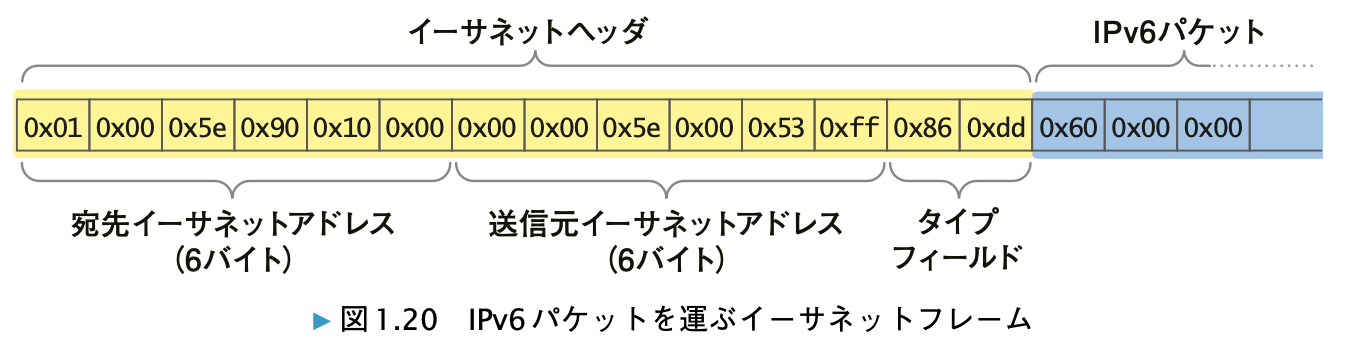
\includegraphics[width=0.99\textwidth]{img/figure1_20.png}
        \end{figure}
      \end{center}
    \end{column}
    \begin{column}{0.5\textwidth}
      \begin{itemize}
        \item よって宛先IPアドレスからMAC(L2アドレス)が解決可能かどうかが重要になる

        \item この近隣探索プロトコルによって、IPアドレスからリンク内のルータやノードのMACアドレスを取得したい
      \end{itemize}
    \end{column}
  \end{columns}
  \begin{itemize}
    \item ついでにMTU(パケットのサイズ?)の設定やリンク内に存在するIPアドレスの範囲も知りたい
  \end{itemize}
\end{frame}

\begin{frame}
  \frametitle{プロトコルで利用するメッセージ(6.1)}

  \begin{itemize}
    \item 近隣探索プロトコルはICMPv6のメッセージ(= IPv6のペイロード)として下記を用いる
    \begin{itemize}
      \item \emph{Router Advertisement} / \emph{Router Solicitation}
      \item \emph{Neighbor Solicitation} / \emph{Neighbor Adovertisement}
      \item Redirect
    \end{itemize}

    \item 近隣探索プロトコルはリンク内で利用されることを前提としているため、
    IPv6のHop Limitを\texttt{255}にしておき、\texttt{255}でなければルータを越えたとして破棄する
    \begin{itemize}
      \item よってICMPv6はIPv6に強く依存しており、このことからL3に分類されるのかもしれない\ce{:thinking:}
    \end{itemize}
  \end{itemize}
\end{frame}

\section{ルータとの近隣探索プロトコル}

\begin{frame}
  \frametitle{%
    ルータとプレフィックス情報\footnote{ルータを経由せずに到達できるIPv6アドレスの範囲のこと。} の発見(6.2)%
  }

  \begin{itemize}
    \item 最初の要約の最初3つだと思う
    \begin{enumerate}
      \item リンク上のルータを探す機能
      \item ルータを経由せずに到達できるIPv6アドレスの範囲を知る機能
      \item リンクのMTUなどの情報を知る機能
    \end{enumerate}

    \item メッセージ``Router Advertisement''と``Router Solicitation''の2つを利用する
  \end{itemize}
\end{frame}

\begin{frame}
  \frametitle{ルータとプレフィックス情報の発見(6.2)}

  \begin{itemize}
    \item ルータはRouter Advertisementメッセージを定期的にノードへマルチキャスト%
    \footnote{マルチキャストでは送信者はネットワークのどこにいてもよく、受信者は複数存在する可能性がある。}する
    \begin{center}
      \begin{figure}
        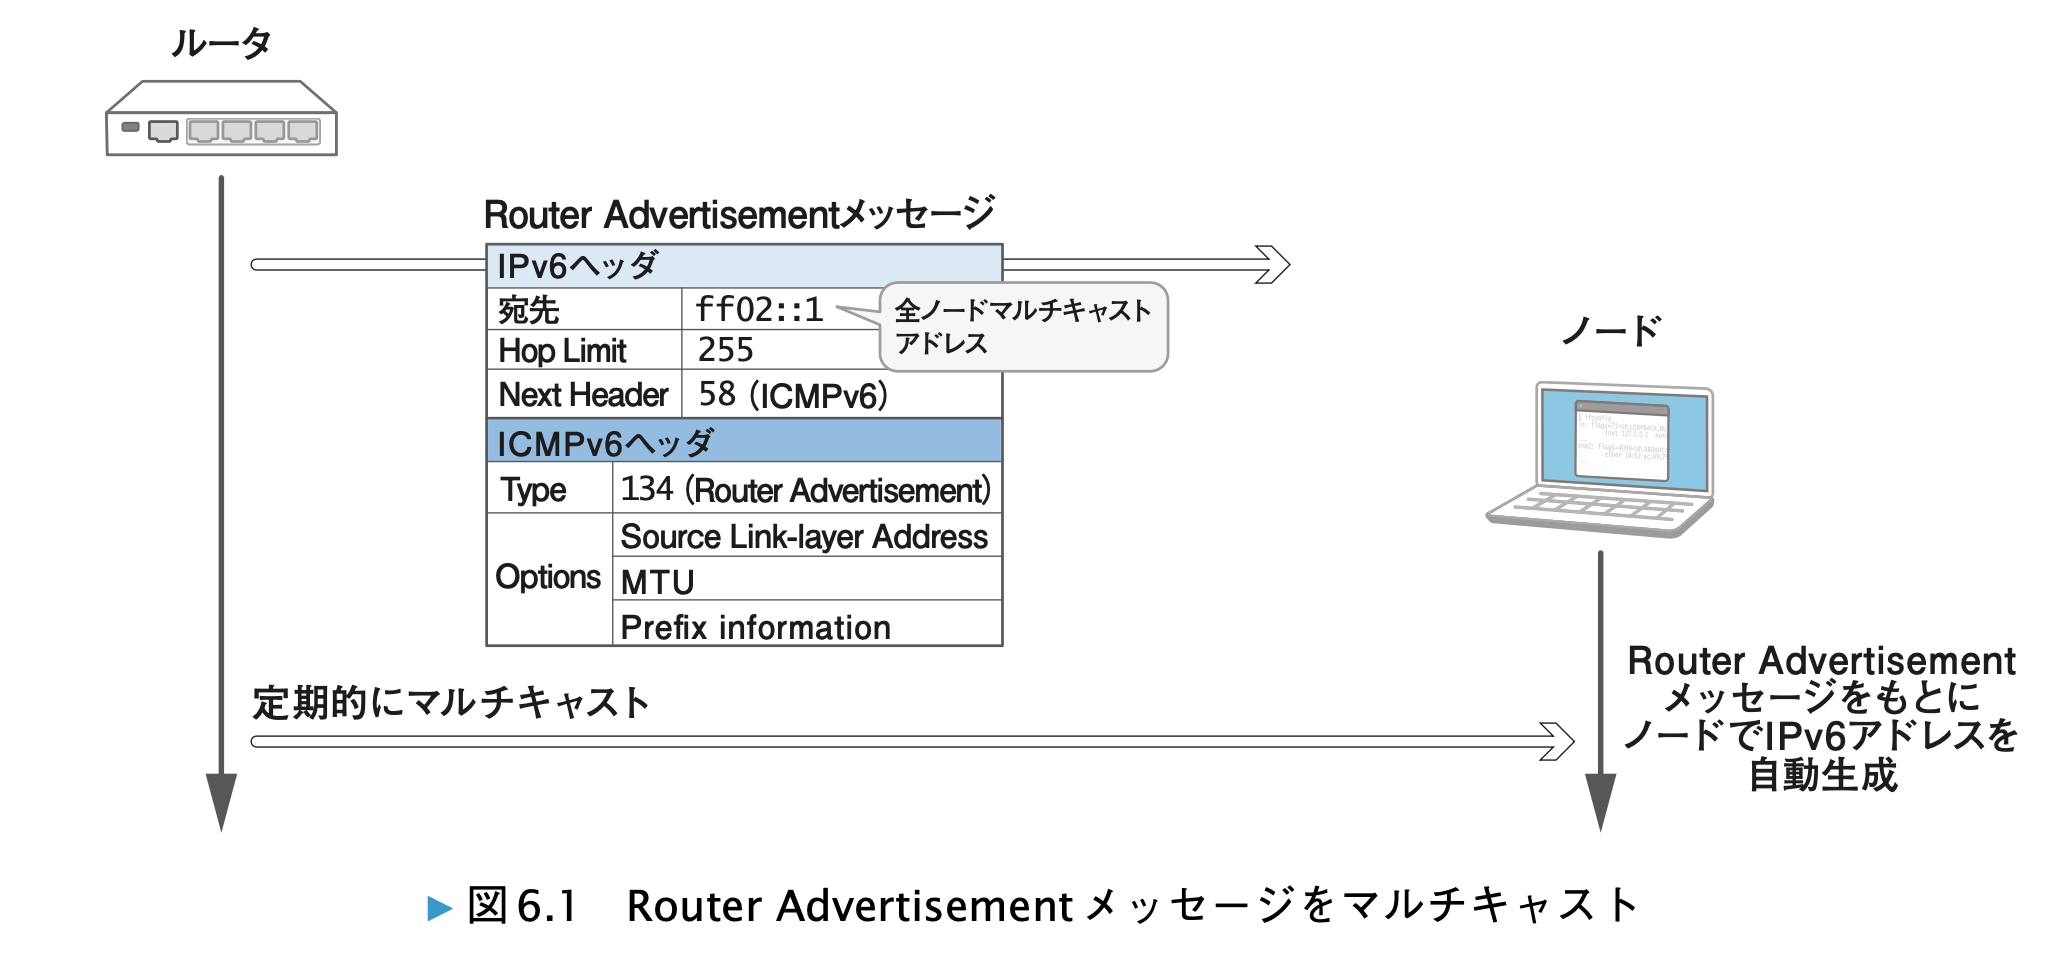
\includegraphics[width=0.5\textwidth]{img/figure6_1.png}
      \end{figure}
    \end{center}

    \item OptionsのところにMACアドレスなどのデータがはいっている

    \item ノードはRouter Solicitationメッセージをルータへ送信することで、
    Router Advertisementを要求することもできる
  \end{itemize}
\end{frame}

\begin{frame}
  \frametitle{Router Advertisementメッセージ(6.2.1)}
  \begin{center}
    \begin{figure}
      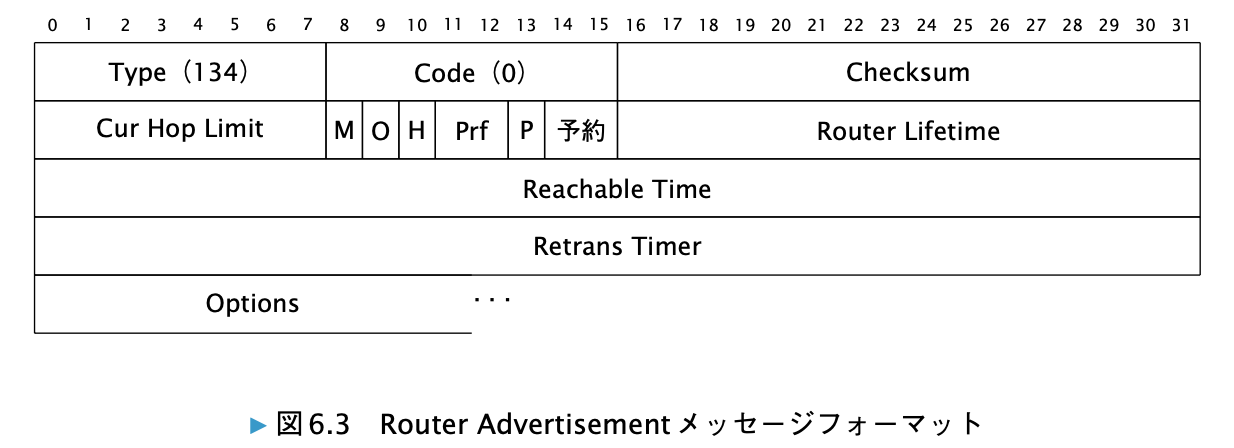
\includegraphics[width=0.65\textwidth]{img/figure6_3.png}
    \end{figure}
  \end{center}

  \begin{itemize}
    \item Optionに含められるのはたとえば次のものがある(RFC 4861, 8106)
    \begin{center}
      \begin{columns}
        \begin{column}{0.4\textwidth}
          \begin{itemize}
            \item Source Link-layer Address
            \item MTU
            \item Prefix Information
          \end{itemize}
        \end{column}
        \begin{column}{0.4\textwidth}
          \begin{itemize}
            \item RDNSS
            \item DNSSL
          \end{itemize}
        \end{column}
      \end{columns}
    \end{center}
  \end{itemize}
\end{frame}

\begin{frame}
  \frametitle{オプションとリンク層アドレス(6.5.2)}

  \begin{itemize}
    \item 下記のようにTLV(Type Length Value)フォーマットでリンク層アドレスを伝搬する
    \begin{center}
      \begin{figure}
        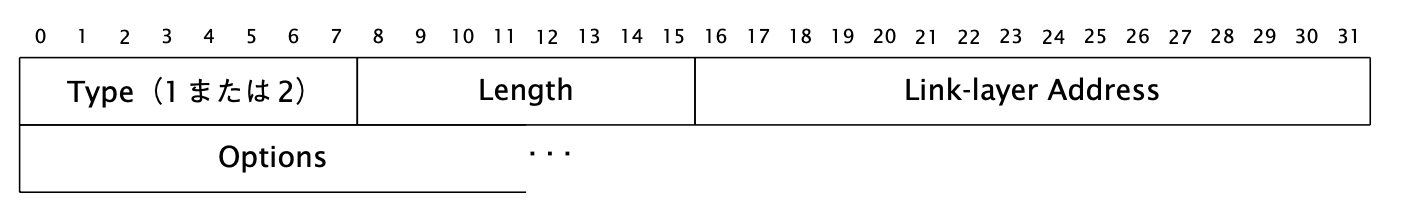
\includegraphics[width=0.65\textwidth]{img/figure6_9.png}
      \end{figure}
    \end{center}
    \begin{description}
      \item[Type] Source Link-layer Addressオプションの場合は1、Target Link-layer Addressオプションの場合は2      
    \end{description}
  \end{itemize}
\end{frame}

\begin{frame}
  \frametitle{ルータ側の処理(6.2.3)}

  \begin{itemize}
    \item デフォルトルータであるかどうかは、Router Lifetimeフィールドを用いて示す

    \item ルータをシャットダウンするなどの理由により送信をやめる場合は、Router Advertisementの
    Router Lifetimeフィールドをゼロに設定して送信するべきとなっている
    
    \item Router AdvertisementメッセージがリンクのMTUを超えてしまう場合、
    オプションを部分的に含んだ複数のRouter Advertisementメッセージに分けて送信することも可能
  \end{itemize}  
\end{frame}

\begin{frame}
  \frametitle{Router Solicitationメッセージ(6.2.2)}

  \begin{itemize}
    \item IPv6ノード側からルータに対してRouter Advertisementをただちに送信するように要求するために用いる
    \begin{center}
      \begin{figure}
        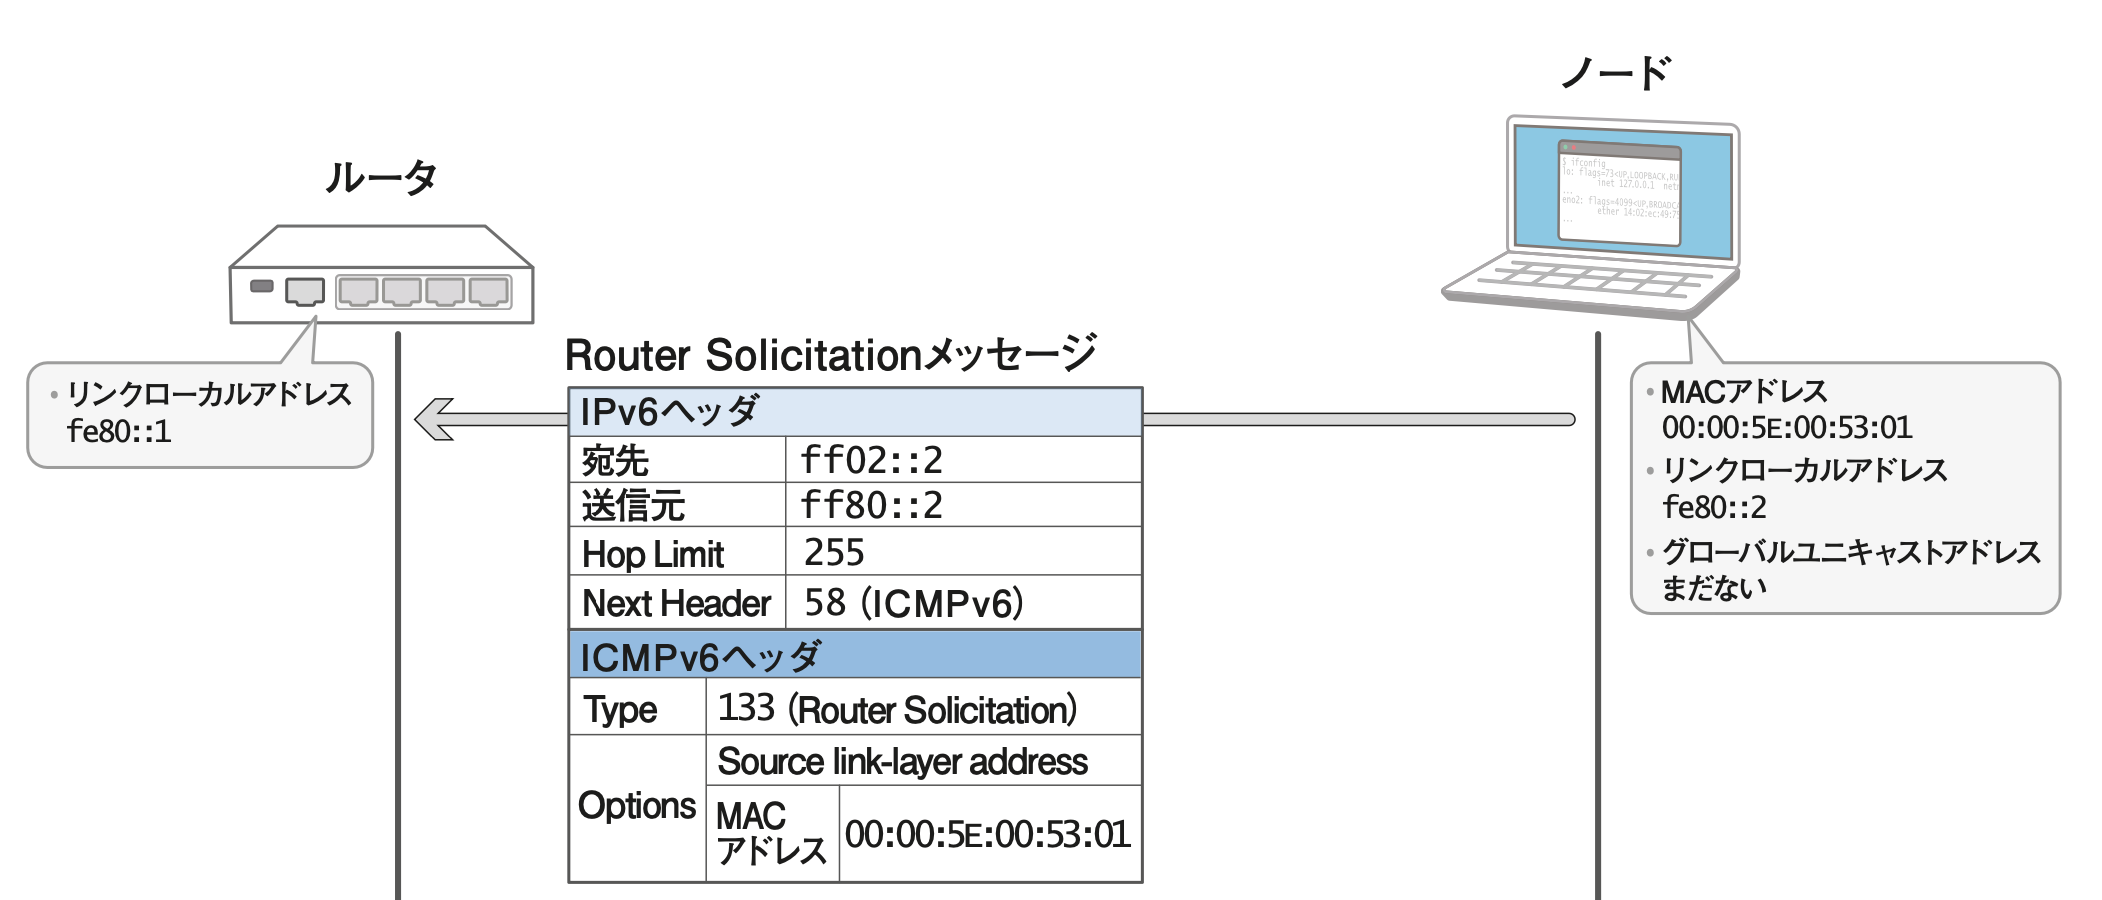
\includegraphics[width=0.55\textwidth]{img/figure6_2.png}
      \end{figure}
    \end{center}

    \item 宛先は通常全ルータへのマルチキャストアドレス\lstinline|ff02::2|となり、
    送信元はリンクローカルアドレスとなる
    \begin{itemize}
      \item IPv6アドレス自動設定でまだIPアドレスがない場合は未定義アドレス\lstinline|::/128|を使う
    \end{itemize}
  \end{itemize}
\end{frame}

\begin{frame}
  \frametitle{Router Solicitationメッセージ(6.2.2)}

  \begin{center}
    \begin{figure}
      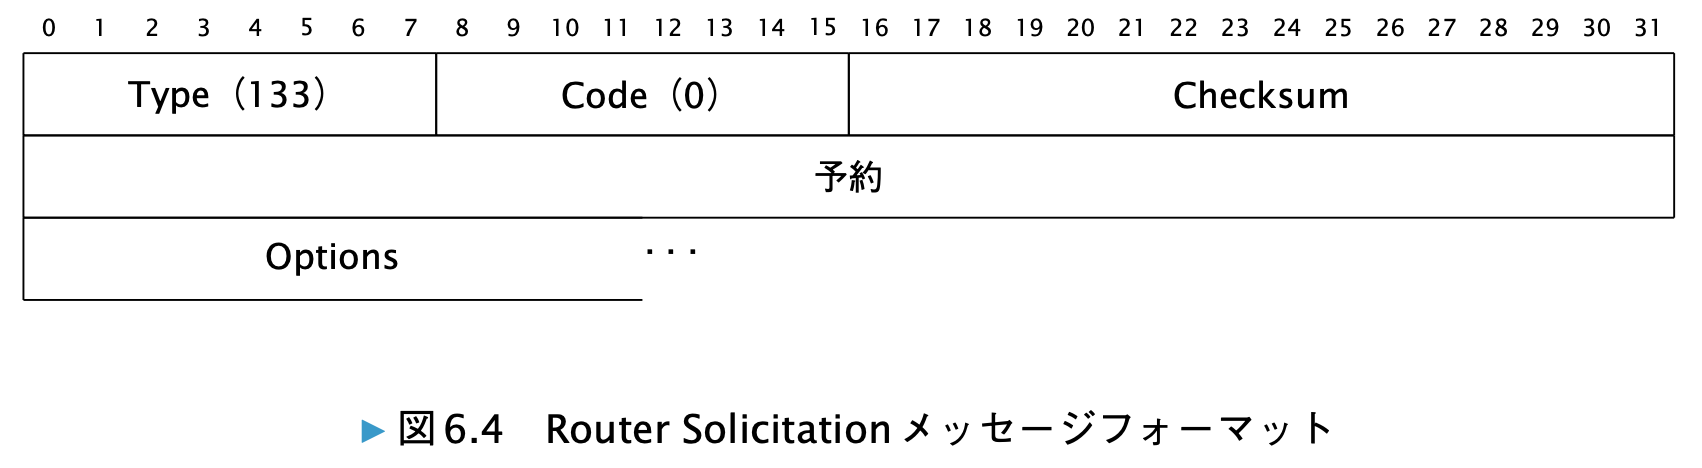
\includegraphics[width=0.65\textwidth]{img/figure6_4.png}
    \end{figure}
  \end{center}

  \begin{itemize}
    \item OptionはSource Link-layer Addressのみ
  \end{itemize}
\end{frame}

\begin{frame}
  \frametitle{ホスト側の処理(6.2.4)}

  \begin{itemize}
    \item ルータではないホストがRouter Advertisementメッセージを送信することは禁止

    \item ホストがRouter Solicitationメッセージを受け取った場合には、何もせずに破棄する(RFC 4861)

    \item ホストはルータがデフォルトルータとしての有効期限(Router Lifetime)が過ぎる前に
    新たなRouter Advertisementメッセージによって有効期限を更新しない場合、
    自身の``Default Router List''からそのルータに関するエントリを削除する
  \end{itemize}
\end{frame}

\section{ノード間の近隣探索プロトコル}

\begin{frame}
  \frametitle{リンク層アドレスの解決と近隣不到達性の検知(6.3)}

  \begin{itemize}
    \item IPv4ではARPでやっていたが、IPv6ではICMPv6の
    Neighbor SolicitationメッセージとNeighbor Advertisementメッセージを利用する

    \item Neighbor SolicitationメッセージとNeighbor Advertisementメッセージは、SLAACの
    DAD(Duplicate Address Detection、重複アドレス検知)でも利用される
  \end{itemize}
\end{frame}

\begin{frame}
  \frametitle{Solicited-Nodeマルチキャストアドレスグループ(6.3.3)}

  \begin{itemize}
    \item ``Solicited-Nodeマルチキャストアドレス''は、
    特定のIPv6アドレスに関連付けられたリンク層アドレスを決定するために近隣探索プロトコルによって使用されるIPv6マルチキャストアドレス

    \item おそらく\textbf{Solicited-Nodeマルチキャストアドレスグループ}はリンク内の全てのノードになるのか?\ce{:thinking:}
  \end{itemize}
\end{frame}

\begin{frame}
  \frametitle{Neighbor Solicitation/Advertisementメッセージ(6.3.1, 2)}

  \begin{itemize}
    \item Neighbor Solicitationメッセージは、リンク層アドレスの解決を行う場合にはSolicited-Nodeマルチキャストで送信
    \begin{itemize}
      \item Optionにリンク層アドレスが入っている
    \end{itemize}

    \item Neighbor Solicitationを受けとったノードは自分のリンク層アドレスをNeighbor Advertisementメッセージで返答する
  \end{itemize}
\end{frame}

\begin{frame}[fragile]
  \frametitle{近隣キャッシュ(6.3.4)}

  \begin{columns}
    \begin{column}{0.7\textwidth}
      \begin{minipage}{\columnwidth}
        \begin{plantuml}
          @startuml

          actor NodeA AS "Node A"
          actor NodeB AS "Node B"
          actor NodeC AS "Node C"

          autonumber

          NodeA -> NodeA: パケットを送りたいNodeBのIPv6アドレスのリンク層アドレスが分かるか?
          alt NodeBのリンク層アドレスが近隣キャッシュにある
            NodeA -> NodeB: パケット送信
          else わからない
            NodeA -> NodeB: Neighbor Solicitationを送信
            NodeA -> NodeC: Neighbor Solicitationを送信
            NodeA -> NodeA: 近隣キャッシュにNodeBのIPアドレスをIMCOMPLETEで保存
            NodeB --> NodeA: Neighbor Advertisementを返信
            NodeC --> NodeA: Neighbor Advertisementを返信

            alt Neighbor Advertisementの送信元IPアドレスがNodeBである
              NodeA -> NodeA: 近隣キャッシュのNodeBのリンク層アドレスを更新
            else 異なる
              NodeA -> NodeA: パケットを破棄
            end
          end
          @enduml
        \end{plantuml}
      \end{minipage}
    \end{column}
    \begin{column}{0.3\textwidth}
      \begin{itemize}
        \item 近隣キャッシュはIPv6アドレスとリンク層アドレスの辞書

        \item 返ってきたNeighbor Advertisementのうち送信元が狙ったIPアドレスだけを
        近隣キャッシュ更新に用いる
      \end{itemize}
    \end{column}
  \end{columns}
\end{frame}

\begin{frame}
  \frametitle{近隣不到達性検知(6.3.5)}
 
  \begin{itemize}
    \item 本では\ce{:point_down:}のようにあるが、これは到達可能性のはなし?\ce{:thinking:}
    \begin{itemize}
      \item 近隣不到達性検知では、自ノードから送ったIPv6パケットを受け取ったことを知らせる何らかの通知を相手ノードから受け取ったときに、その相手ノードへは到達可能であると判断します
    \end{itemize}

    \item ようするにNeighbor Solicitationを送ったけど、狙ったIPアドレスから返答がなかったということ?
  \end{itemize}
\end{frame}

\begin{frame}
  \frametitle{近隣キャッシュのステート(6.3.6)}
  
  \begin{itemize}
    \item いろいろある
  \end{itemize}
\end{frame}

\section{Redirect}

\begin{frame}
  \frametitle{Redirectメッセージ(6.4)}

  \begin{itemize}
    \item Redirectメッセージはルータからホストへ次のようなときに送信される
    \begin{itemize}
      \item 他のルータが特定の経路としてより良い次ホップであることをルータからホストに対して伝えるとき
      \item 特定の宛先が実際には同一リンク上に接続された近隣ノードであることを伝えるとき
    \end{itemize}

    \item IPv6はリンク内に複数のルータがあるから、そういうこともある?\ce{:thinking:}
    \begin{center}
      \begin{figure}
        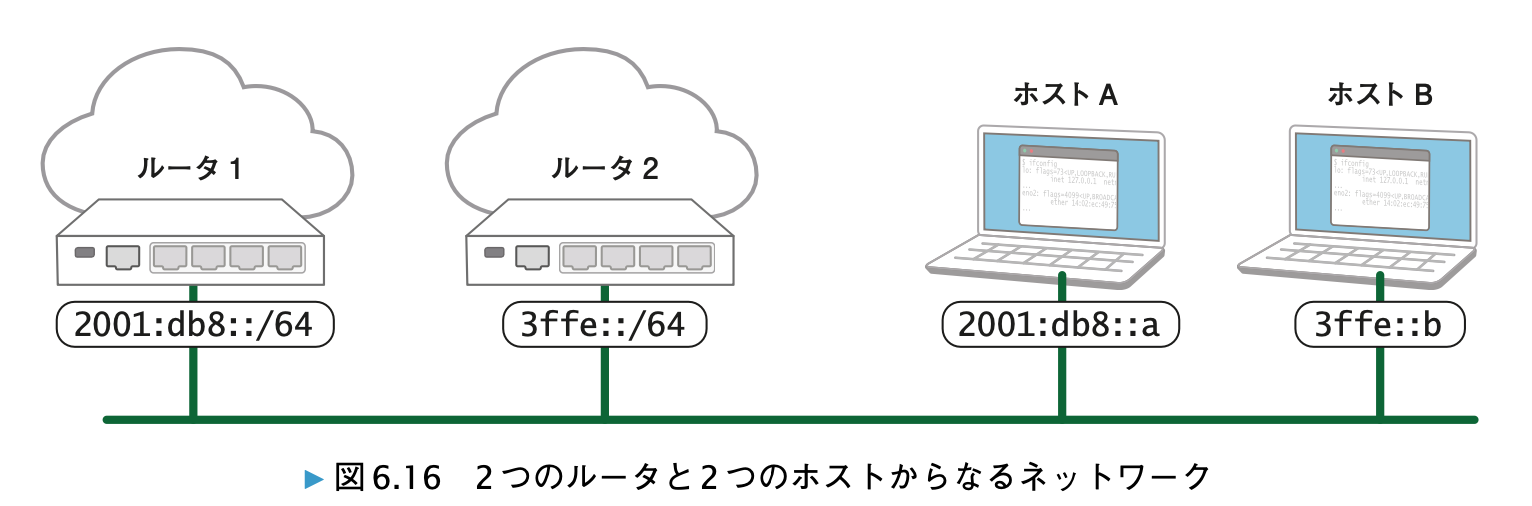
\includegraphics[width=0.65\textwidth]{img/figure6_16.png}
      \end{figure}
    \end{center}
  \end{itemize}
\end{frame}

\section{on-linkとoff-link}

\begin{frame}
  \frametitle{on-linkとoff-link(6.6)}

  \begin{center}
    \begin{figure}
      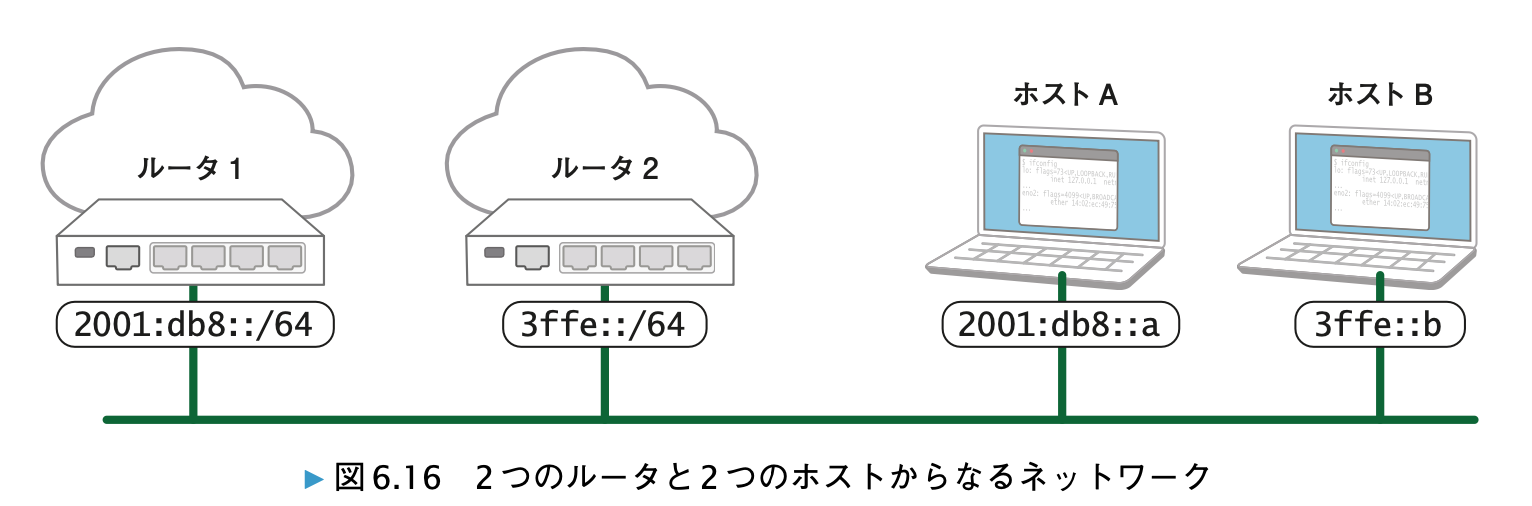
\includegraphics[width=0.55\textwidth]{img/figure6_16.png}
    \end{figure}
  \end{center}

  \begin{itemize}
    \item 同一リンクに接続されていることをon-link、同一リンクに接続されていないことをoff-linkと表現する

    \item IPv6ではIPアドレスとプレフィックスによりon-linkかどうかを決定できない
    \begin{itemize}
      \item IPv4はできたが、IPv6は1つのネットワークインターフェースに複数のIPv6アドレスが設定できるためできない
    \end{itemize}

    \item たとえば上の図であれば、プレフィックスは異なるがホストAからホストBはon-linkである
    %\begin{itemize}
    %  \item 別プレフィックスでoff-linkと判断すると、ホストA→ホストBはルータ2を経由する必要がある
    %\end{itemize}
  \end{itemize}
\end{frame}

\begin{frame}
  \frametitle{on-link情報(6.6.1)}

  \begin{itemize}
    \item Router Advertisementにあるプレフィックス情報を使う

    \item Redirectメッセージが示すTarget Addressがリンクローカルアドレスではなく、
    かつDestination AddressがTarget Addressと同じものであるとき、
    そのメッセージはTarget Addressで示される宛先がon-linkであることを示す
  \end{itemize}
\end{frame}

\section*{References}
\begin{frame}%[allowframebreaks]
  \frametitle{References}
  % \nocite{*}
  \bibliographystyle{junsrt_url}
  \bibliography{ref}
\end{frame}

\begin{frame}
  \centering
  {\Huge Thank you for the attention!}
\end{frame}

\end{document}
